\section{Experiments and Discussion}

To mimic the process of querying an API, we simulate sampling from an existing network dataset. We compare our algorithm with the MOD algorithm\cite{avrachenkov2014pay}. For simplicity, we assume all networks are undirected. We use four different datasets, described in Table \ref{tab:dataset}. $\textit{Grad}$ and $\textit{Undergrad}$ are the Facebook networks \cite{mislove2010you}. $\textit{Enron-Email}$ is an email communication network. $Twitter$ is a friend-follower network that we collected via Twitter API.

\begin{table}
\centering
 %\captionof{table}{Names and statistics of datasets used in our work.} \label{tab:dataset} 
 	\caption{Names and statistics of datasets used in our work.}
 	\label{tab:dataset} 
    \begin{tabular}{ l | c | c | c | c }
    \hline
	 Network & \# Nodes & \# Edges & Global CC. & Mod. \\ \hline
	 Grad & 503 & 3256 & 0.4792 & 0.6915 \\
	 Undergrad & 1220 & 43208 & 0.2980 & 0.3937 \\
	 Twitter & 12230 & 50884 & 0.1117 & 0.6371 \\
	 Enron-Email & 36692 & 183831 & 0.4970 & 0.5975 \\ \hline
    \end{tabular}
   
\end{table}

\begin{figure}[h]
 	\centering
    \begin{subfigure}[t]{0.25\textwidth}
        \centering
        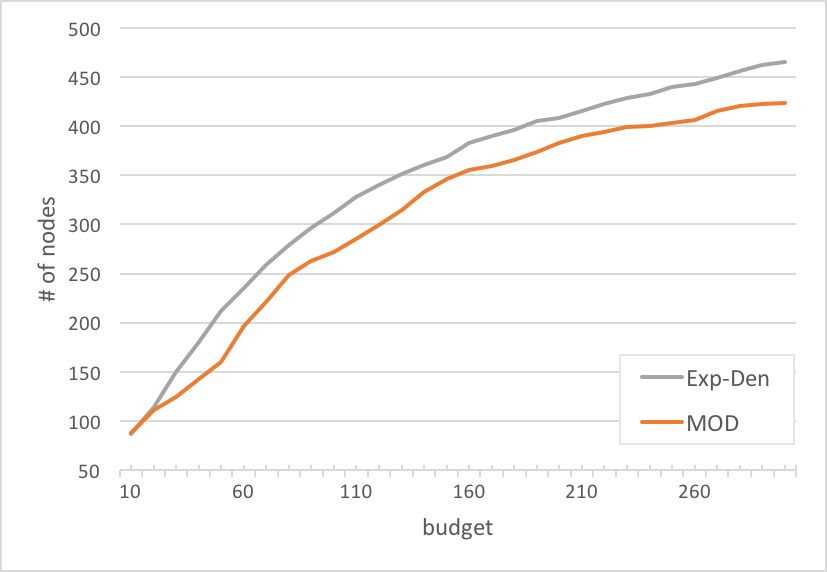
\includegraphics[height=1.1in]{grad2}
        \caption{Grad}
    \end{subfigure}%
    ~ 
    \begin{subfigure}[t]{0.25\textwidth}
        \centering
        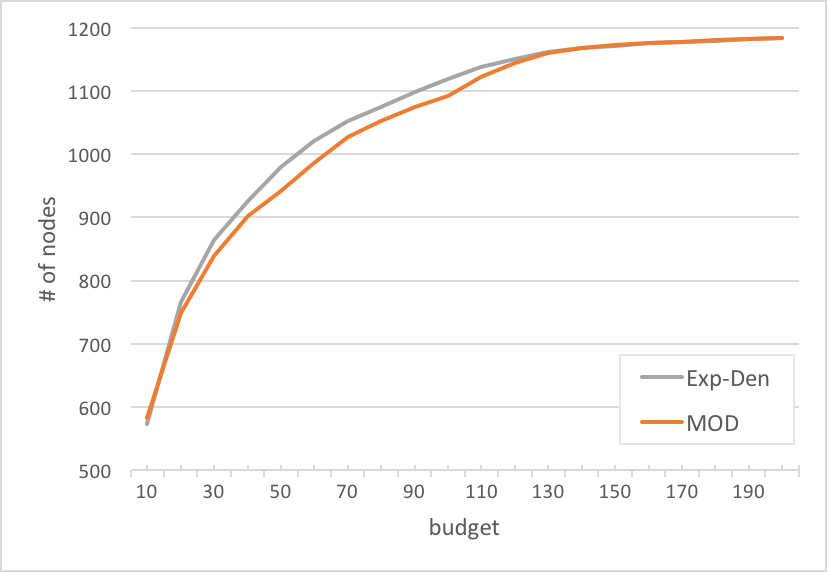
\includegraphics[height=1.1in]{undergrad2}
        \caption{Undergrad}
    \end{subfigure}
     \begin{subfigure}[t]{0.25\textwidth}
        \centering
        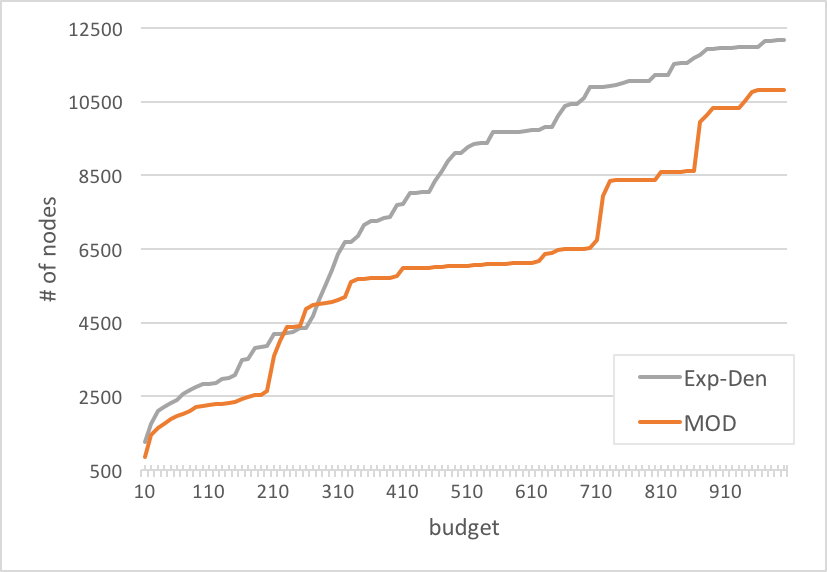
\includegraphics[height=1.1in]{twitter2}
        \caption{Twitter}
    \end{subfigure}%
    ~ 
    \begin{subfigure}[t]{0.25\textwidth}
        \centering
        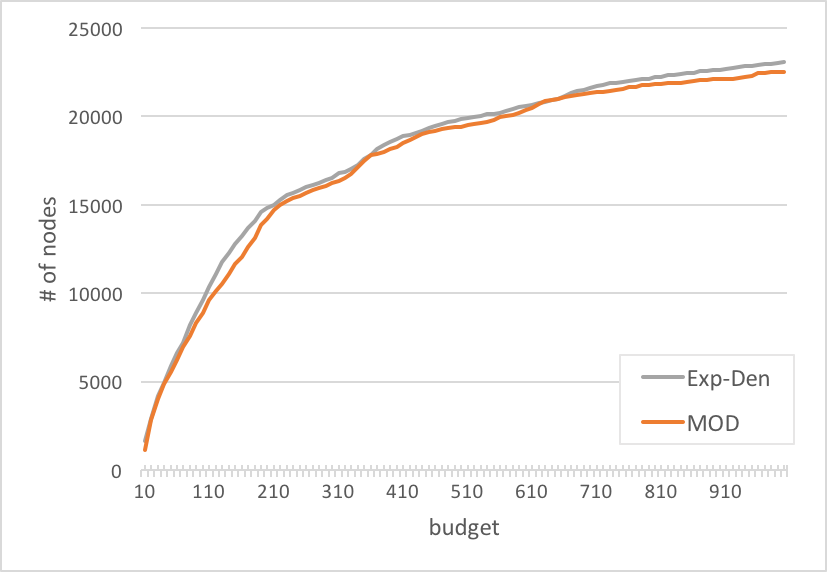
\includegraphics[height=1.1in]{enron2}
        \caption{Enron-Email}
    \end{subfigure}
   	 \caption{Experimental results on each dataset}\label{fig:result}
\end{figure}

We ran 15 experiments on each dataset, and plotted average values in Figure \ref{fig:result}. These plots depict the between amount of budget used versus the number of nodes obtained. Our algorithm outperformed MOD in every case. This gives us strong evidence that \ref{algo-name} algorithm is able to collect more nodes than MOD at the same amount of budget.  Interestingly, on the Twitter dataset, we clearly see that MOD becomes trapped in a region before being forced into a new region (indicated by steps in the result curve). A large budget is spent, but few nodes are added to the sample.

With a budget constraint, \ref{algo-name} performs well. Our future work includes improving the Expansion strategy with different switching criteria. 

%A criteria for switching between Densification and Expansion needs more studies.